\begin{center}
\hyperdef{}{OLEux5fLINK7}{}{\hyperdef{}{OLEux5fLINK8}{}{}}Oliver R.
Hoidn and Gerald T. Seidler

\hyperdef{}{OLEux5fLINK9}{}{}\emph{Physics Department, University of
Washington, Seattle WA 98195}
\end{center}


\hyperdef{}{OLEux5fLINK5}{}{\hyperdef{}{OLEux5fLINK6}{}{}}
\section{Abstract}
We have integrated mass-produced commercial complementary
metal-oxide-semiconductor (CMOS) image sensors and off-the-shelf
single-board computers into an x-ray camera platform optimized for
acquisition of x-ray spectra and radiographs at energies of 2 -- 6 keV.
The CMOS sensor and single-board computer are complemented by custom
mounting and interface hardware that can be easily acquired from rapid
prototyping services. For single-pixel detection events, i.e., events
where the deposited energy from one photon is substantially localized in
a single pixel, we establish $\sim$120\% quantum efficiency at
2.6 keV with $\sim$190 eV resolution and a 100 kHz maximum
detection rate. The detector platform's useful intrinsic energy
resolution,
\hyperdef{}{OLEux5fLINK12}{}{\hyperdef{}{OLEux5fLINK13}{}{\hyperdef{}{OLEux5fLINK14}{}{}}}5-µm
pixel size, ease of use, and obvious potential for parallelization make
it a promising candidate for many applications at synchrotron
facilities, in laser-heating plasma physics studies, and in
laboratory-based x-ray spectrometry.


\section{Introduction}
\hyperdef{}{OLEux5fLINK18}{}{\hyperdef{}{OLEux5fLINK19}{}{}}The
performance of a wide range of contemporary applications of x-ray
methods are contingent upon the capabilities of x-ray imaging sensors.
Examples include radiographic imaging across the full span of spatial
resolutions in addition to both energy-dispersive and
wavelength-dispersive spectroscopy in
astrophysics\hyperref[ux5fENREFux5f1]{\textsuperscript{1-3}}, plasma
physics\hyperref[ux5fENREFux5f4]{\textsuperscript{4-6}}, synchrotron
science\hyperref[ux5fENREFux5f7]{\textsuperscript{7-11}}, and
laboratory-based x-ray
spectroscopies\hyperref[ux5fENREFux5f12]{\textsuperscript{12}}. The
growing centrality of imaging detectors, especially those with
significant single-pixel energy resolution, has led to a steady increase
in commercial products and also niche-specific research efforts.

Here, we are most interested in a particular endpoint of these efforts,
the possibility of mass-production of disposable x-ray spectroscopic
cameras, i.e., those where each pixel has some significant energy
resolution, having good performance for 2 -- 6 keV photon energies. The
ready availability of such sensors would be beneficial in several of the
fields mentioned above while also serving as an easy test platform for
new applications and as a convenient tool in education. We are not the
first to consider these issues, and recent work in this subfield has
demonstrated tantalizing potential for spectroscopic cameras based on
standard, consumer-grade monochrome complementary metal-oxide
semiconductor (CMOS) pixel
arrays,\hyperref[ux5fENREFux5f13]{\textsuperscript{13-15}} such as
regularly used in security cameras and other low-end imaging
applications. This prior work establishes the viability of CMOS pixel
arrays as spectroscopic imaging detectors of hard x rays and explores a
host of performance characteristics, including linearity,
radiation-hardness, and spatial response to single-photon interactions.
The use of CMOS sensors, instead of charge-coupled devices (CCDs), is
motivated by their lower cost due to chip-level integration of all
sensor functions and the mature state of CMOS fabrication technology, as
well as their typically much higher radiation
hardness\hyperref[ux5fENREFux5f16]{\textsuperscript{16}}\emph{.} These
considerations are in some ways representative of other efforts where
admittedly much more advanced and specialized CMOS sensors are making
growing inroads. \hyperref[ux5fENREFux5f17]{\textsuperscript{17}}

\section{Methods, Results, and Discussion}
Unlike prior work, here we investigate sensor performance below 6 keV
photon energy. Our sensor platform design is driven by the goals of: (1)
achieving a high saturation count rate, (2) generating single-photon
spectra in real time, (3) ease of operation for new
wavelength-dispersive spectrometer development in the laboratory
setting\hyperref[ux5fENREFux5f18]{\textsuperscript{18}} and (4)
developing simple sensor exchange to make the camera viable as a
disposable detector for use in plasma physics experiments where
experimental diagnostics are exposed to large electromagnetic pulses and
to hazards from shrapnel from the laser-target interaction.

We consequently avoid commercial camera bodies and sensor evaluation
boards, instead using a mass-produced CMOS sensor that can be easily and
inexpensively replaced if damaged, a general-purpose single-board
computer (SBC) having fast and flexible GPI/O capability as the
principal hardware component, and a custom sensor board that has been
designed in-house and fabricated by a rapid-prototyping printed circuit
board service. To be specific, the sensor is an Aptina MT9M001
monochrome CMOS device with 1280 x 1024 resolution and a pixel size of
5.2 x 5.2 µm\textsuperscript{2}. The sensor was chosen primarily because
of its high near-infrared sensitivity, which indicates a relatively
thick active layer. Before the chip's installation its protective glass
cover was removed, as it strongly absorbs x rays. The SBC is similarly a
mass-produced component (BeagleBone Black SBC, Texas Instruments). The
SBC is based on the AM3358 system on a chip, which contains an ARM
Cortex A8 processor and a PRU-ICSS (Programmable Real-Time Unit
Subsystem and Industrial Communication SubSystem) subsystem with two
Programmable Realtime Unit (PRU) coprocessors. The SBC's software
interface to the sensor board consists of two PRU programs (implemented
in PRU assembler) that perform the readout and communicate with a Linux
user space program (implemented in C) that concurrently processes the
resulting data stream (see Fig. 1). The PRUs operate at 200 million
instructions per second (MIPS) and are configured for single-clock
access to the GPI/O pins on the SBC that interface with the sensor PCB.
This is sufficient for readout at 30 frames per second (fps), near the
MT9M001's maximum data rate. Our current implementation suffers from a
memory bandwidth bottleneck that restricts frame rate to 10 fps, but
this limitation can be removed by improving the PRU Linux kernel
driver's allocation and management of the ARM/PRU DDR buffer so that it
exploits the ARM core's CPU cache.

\begin{figure}[h] \label{cm1image1}
\caption{ Block diagram of the CMOS camera design.}
\centering
\hyperdef{}{OLEux5fLINK1}{}{}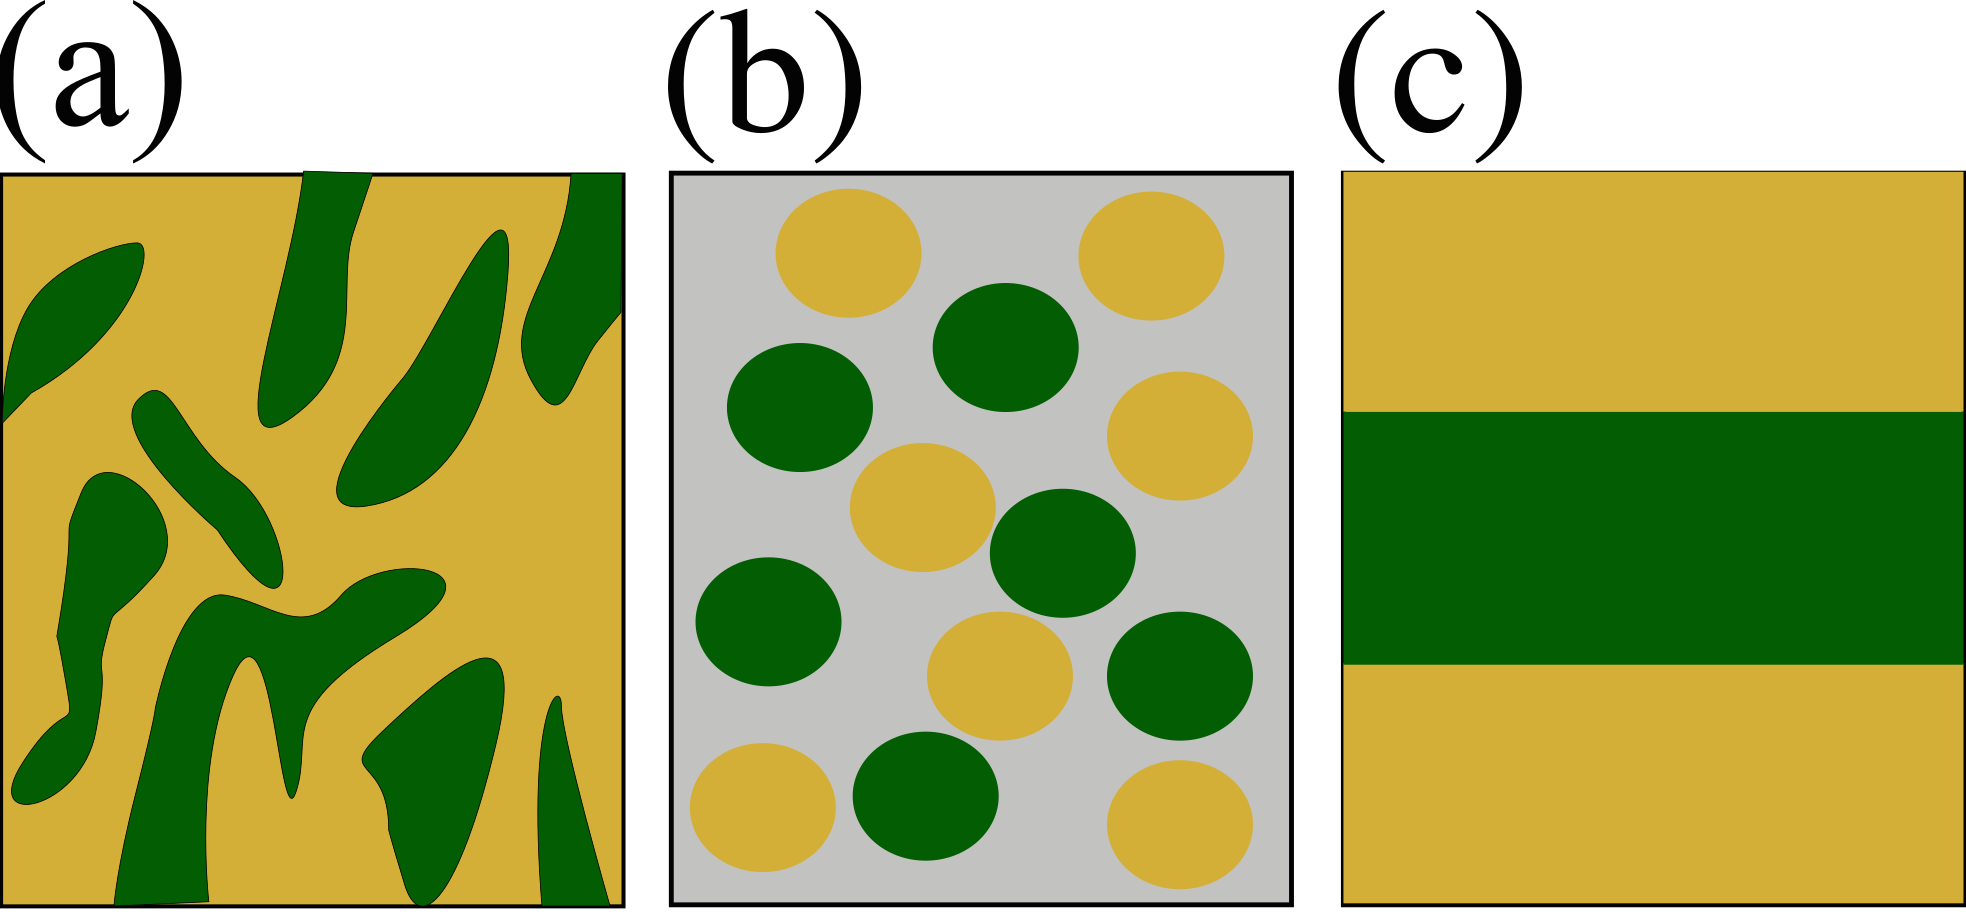
\includegraphics{cmos1/image1.png}
\end{figure}

\begin{figure}[h] \label{cm1image2}
\caption{ (a) An image of the camera,
and (b) the camera's quantum efficiency in single-photon counting mode
as a function of x-ray photon energy, as established by comparison with
a commercial Si drift detector. The glass cover of the CMOS sensor has
been removed to allow direct x-ray detection.}
\centering
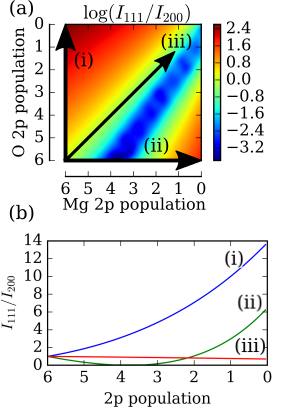
\includegraphics{cmos1/image2.png}
\end{figure}

\FloatBarrier

Multiple steps in processing are all performed on the SBC, and processed
data is stored on the SBC's SD card before transfer to the control
workstation. An exposure sequence accumulates the sum of all individual
frames as a single image. Additionally, a spectrum is generated by
binning the number of pixels per ADC channel. The finest energy
resolution requires operating the sensor in the low-intensity single
photon counting (SPC) regime where the mean period between photons
incident on a given pixel is significantly larger than the frame time.
Only x-ray events for which the entire charge cloud is concentrated in a
single pixel are incorporated into the spectrum; this filtering step,
which we refer to as cluster rejection, is well-established as necessary
for optimal performance in pixel detectors used for SPC
spectroscopy\hyperref[ux5fENREFux5f13]{\textsuperscript{13}}\textsuperscript{,}
\hyperref[ux5fENREFux5f19]{\textsuperscript{19}}.
\hyperdef{}{OLEux5fLINK38}{}{\hyperdef{}{OLEux5fLINK39}{}{\hyperdef{}{OLEux5fLINK40}{}{\hyperdef{}{OLEux5fLINK41}{}{}}}}

In cluster-rejection mode the sensor's saturation rate is 100,000
photons per second, but this can improved $\sim$3-fold by
resolving the aforementioned memory bottleneck. The quantum efficiency
(QE) of the detector was characterized by measurement of the
\emph{K}-shell fluorescence spectra of chlorine, calcium, and several
transition metals. This was done using a low-power laboratory x-ray tube
source to excite 1\emph{s} core holes of these elements in various solid
samples. The intensity of resulting
\hyperdef{}{OLEux5fLINK2}{}{\hyperdef{}{OLEux5fLINK3}{}{\hyperdef{}{OLEux5fLINK4}{}{\hyperdef{}{OLEux5fLINK15}{}{\hyperdef{}{OLEux5fLINK16}{}{\hyperdef{}{OLEux5fLINK17}{}{\hyperdef{}{OLEux5fLINK20}{}{\hyperdef{}{OLEux5fLINK21}{}{\hyperdef{}{OLEux5fLINK22}{}{\hyperdef{}{OLEux5fLINK23}{}{\hyperdef{}{OLEux5fLINK24}{}{\hyperdef{}{OLEux5fLINK25}{}{\hyperdef{}{OLEux5fLINK26}{}{\hyperdef{}{OLEux5fLINK27}{}{\hyperdef{}{OLEux5fLINK28}{}{\hyperdef{}{OLEux5fLINK29}{}{}}}}}}}}}}}}}}}}\(K_{\alpha}\)
and
\hyperdef{}{OLEux5fLINK30}{}{\hyperdef{}{OLEux5fLINK31}{}{\hyperdef{}{OLEux5fLINK32}{}{\hyperdef{}{OLEux5fLINK33}{}{}}}}\(K_{\beta}\)
emission registered by the detector was referenced to that recorded at
the same position by a commercial Si drift detector (Amptek XR-100SDD)
having known QE; results are presented in Fig. 2. Due to the small
active layer thickness of the CMOS sensor, its quantum efficiency
rapidly decreases from 19\% at 2.6 keV (Cl \(K_{\alpha}\) emission) to
$\sim$1\% at 8.0 keV (Cu \(K_{\alpha}\) emission). For
imaging applications, such as use as a position-sensitive detector in
wavelength-dispersive spectroscopy, it is clear that higher QE can be
obtained by cluster identification, i.e., including information from
events with some multipixel character. Our initial experience suggests a
50\% increase in detected photon rate, but this requires further
investigation. We expect that the QE will decrease below the Si
\emph{K}-edge because of the sudden increase in penetration length
compared to the active layer thickness, but that some utility will
remain below 1.5 keV. The present camera design is being modified for
easier vacuum compatibility and the above issue will be investigated.

We now present detector performance in two representative applications.
The radiograph in Fig. 3 (a) demonstrates the sensor's use as an imaging
detector, while Fig. 3 (b) presents a spectrum of Mn \emph{K}-shell
emission. No dark-field corrections are used here: the dark counts are
negligible in this bin range. The FWHM of the sensor's energy response
function at Mn \(K_{\alpha}\) is 280 eV, approximately two times as
large as in Fano noise-limited x-ray CCDs but still sufficiently small
for the Mn \(K_{\alpha}\) and \(K_{\beta}\) emission peaks to be
resolved. The resolution generally scales as \(\sqrt{E}\), where
\emph{E} is photon energy, for example showing 190 eV resolution at Cl
\hyperdef{}{OLEux5fLINK34}{}{\hyperdef{}{OLEux5fLINK35}{}{\hyperdef{}{OLEux5fLINK36}{}{\hyperdef{}{OLEux5fLINK37}{}{}}}}\(K_{\alpha}\)
and 330 eV at Cu \(K_{\alpha}\). The spectrum's background below the Mn
\(K_{\alpha}\) peak energy is due to incomplete collection of charge
from photon events, even after filtering for single-pixel events.

The camera's good QE below 4 keV suggests that few-keV x ray
spectroscopy, whether in direct detection or as the position sensitive
detector in a wavelength-dispersive
instrument\hyperref[ux5fENREFux5f9]{\textsuperscript{9-11}}, would be a
particularly favorable venue. In this regime, the smaller pixel
dimension of CMOS sensors similar to the MT9M001 is a significant
advantage relative to conventional x-ray CCDs, as it enables the
combination of short working distance, high collection solid angle, and
high energy
resolution.\hyperref[ux5fENREFux5f14]{}\hyperref[ux5fENREFux5f10]{\textsuperscript{10}}\textsuperscript{,}
\hyperref[ux5fENREFux5f20]{\textsuperscript{20-22}} Additionally, such
CMOS sensors' much smaller (1\% or under) cost, while not in itself a
technical innovation, makes them promising candidates for disposable
direct-detection spectrometers in laser plasma experiments, for
high-resolution radiography in educational (instructional) settings, ,
and for versatile coverage of special scattering angles in synchrotron
studies.

\begin{figure}[h] \label{cm1image3}
\caption{ (a) Radiograph of a flower petal. The grayscale is a
representation of raw incident intensity. Improved spatial resolution
would be achieved by selection of single-pixel
events\hyperref[ux5fENREFux5f14]{\textsuperscript{14}}. (b) X-ray
emission spectrum of a Mn metal foil excited by a low-power laboratory
x-ray tube source. The spectrum is based only on nominally single-pixel
events.}
\centering
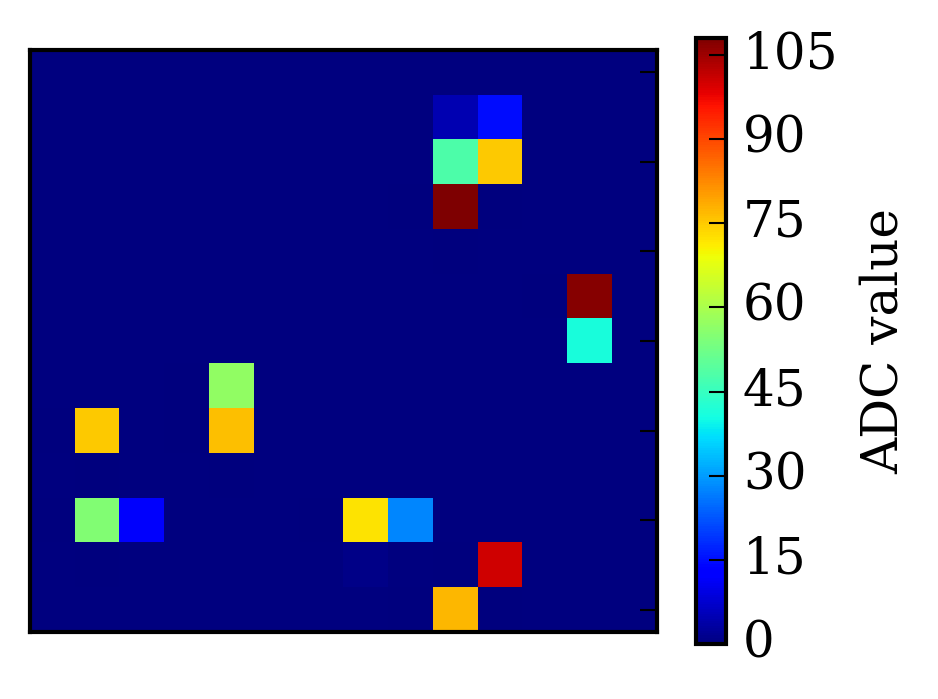
\includegraphics{cmos1/image3.png}
\end{figure}

\FloatBarrier

\section{Conclusions}
We have reported the development of a flexible and
surprisingly effective x-ray camera platform composed of standard
commercial components merged with custom electronics that can be readily
ordered from commercial prototyping services. The observed performance
suggests an interesting range of future applications at photon energies
of a few keV. This includes two aggressive possibilities: (1) large-area
spectroscopic detectors formed by multiplexing large numbers of our
cameras to reach net spectroscopic count rates useful for studies at the
highest-intensity synchrotron beamlines or at x-ray free electron
lasers, and (2) disposable detectors for use in the EMP-rich
environments of laser plasma experiments.

\section{Acknowledgments}: This work was supported by the U.S.
Department of Energy, Basic Energy Sciences under Grant No.
DE-FG02-09ER16106 and also by the Office of Science, Fusion Energy
Sciences and the National Nuclear Security Administration thought Grant
No. DE-SC0008580. We thank Bryan Venema for assistance with board
assembly and for many useful discussions.

\section{References}

\hyperdef{}{ux5fENREFux5f1}{}{}1. K. Koyama, et al., Publications of the
Astronomical Society of Japan \textbf{59} (sp1), S23-S33 (2007).

\hyperdef{}{ux5fENREFux5f2}{}{}2. P. Lechner, R. Hartmann, P. Holl, G.
Lutz, N. Meidinger, R. H. Richter, H. Soltau and L. Strüder, Nuclear
Instruments and Methods in Physics Research Section A: Accelerators,
Spectrometers, Detectors and Associated Equipment \textbf{509} (1--3),
302-314 (2003).

\hyperdef{}{ux5fENREFux5f3}{}{}3. A. Stefanescu, et al., Nuclear
Instruments and Methods in Physics Research Section A: Accelerators,
Spectrometers, Detectors and Associated Equipment \textbf{624} (2),
533-539 (2010).

\hyperdef{}{ux5fENREFux5f4}{}{}4. S. R. Nagel, et al., Review of
Scientific Instruments \textbf{83} (10), 10E116 (2012).

\hyperdef{}{ux5fENREFux5f5}{}{}5. G. R. Plateau, et al., Physical Review
Letters \textbf{109} (6), 064802 (2012).

\hyperdef{}{ux5fENREFux5f6}{}{}6. E. J. Gamboa, C. M. Huntington, M. R.
Trantham, P. A. Keiter, R. P. Drake, D. S. Montgomery, J. F. Benage and
S. A. Letzring, Review of Scientific Instruments \textbf{83} (10),
10E108 (2012).

\hyperdef{}{ux5fENREFux5f7}{}{}7. I. Ordavo, et al., Nuclear Instruments
and Methods in Physics Research Section A: Accelerators, Spectrometers,
Detectors and Associated Equipment \textbf{654} (1), 250-257 (2011).

\hyperdef{}{ux5fENREFux5f8}{}{}8. M. Stampanoni, G. Borchert, P. Wyss,
R. Abela, B. Patterson, S. Hunt, D. Vermeulen and P. Rüegsegger, Nuclear
Instruments and Methods in Physics Research Section A: Accelerators,
Spectrometers, Detectors and Associated Equipment \textbf{491} (1--2),
291-301 (2002).

\hyperdef{}{ux5fENREFux5f9}{}{}9. S. Huotari, F. Albergamo, G. Vankó, R.
Verbeni and G. Monaco, Review of Scientific Instruments \textbf{77} (5),
053102 (2006).

\hyperdef{}{ux5fENREFux5f10}{}{}10. S. Huotari, G. Vanko, F. Albergamo,
C. Ponchut, H. Graafsma, C. Henriquet, R. Verbeni and G. Monaco, Journal
of Synchrotron Radiation \textbf{12} (4), 467-472 (2005).

\hyperdef{}{ux5fENREFux5f11}{}{}11. M. Kavčič, M. Budnar, A. Mühleisen,
F. Gasser, M. Žitnik, K. Bučar and R. Bohinc, Review of Scientific
Instruments \textbf{83} (3), 033113 (2012).

\hyperdef{}{ux5fENREFux5f12}{}{}12. J. Hoszowska, J. C. Dousse, J. Kern
and C. Rhême, Nuclear Instruments and Methods in Physics Research
Section A: Accelerators, Spectrometers, Detectors and Associated
Equipment \textbf{376} (1), 129-138 (1996).

\hyperdef{}{ux5fENREFux5f13}{}{}13. L. Servoli, D. Biagetti, D. Passeri
and E. S. Gattuso, Journal of Instrumentation \textbf{5} (07), P07003
(2010).

\hyperdef{}{ux5fENREFux5f14}{}{}14. F. Nachtrab, T. Hofmann, M.
Firsching, N. Uhlmann and R. Hanke, Nuclear Science Symposium Conference
Record (NSS/MIC), 2009 IEEE, pp. 1636-1639.

\hyperdef{}{ux5fENREFux5f15}{}{}15. D. W. Lane, Nuclear Instruments and
Methods in Physics Research Section B: Beam Interactions with Materials
and Atoms \textbf{284}, 29-32 (2012).

\hyperdef{}{ux5fENREFux5f16}{}{}16. K. Abe, et al., Nuclear Instruments
and Methods in Physics Research Section A: Accelerators, Spectrometers,
Detectors and Associated Equipment \textbf{400} (2), 287-343 (1997).

\hyperdef{}{ux5fENREFux5f17}{}{}17. A. D. Falcone, D. N. Burrows, Y.
Bai, M. Farris, R. Cook and S. Bongiorno, Optical Engineering and
Applications \textbf{6686}, pp. 668602-668606.

\hyperdef{}{ux5fENREFux5f18}{}{}18. G. Seidler, D. Mortensen, A.
Remesnik, J. Pacold, N. Ball, N. Barry, M. Styczinski and O. Hoidn,
Review of Scientific Instruments \textbf{85} (11), 113906 (2014).

\hyperdef{}{ux5fENREFux5f19}{}{}19. B. R. Maddox, H. S. Park, B. A.
Remington and M. McKernan, Review of Scientific Instruments \textbf{79}
(10), 10E924 (2008).

\hyperdef{}{ux5fENREFux5f20}{}{}20. J. I. Pacold, et al., Journal of
Synchrotron Radiation \textbf{19} (2), 245-251 (2012).

\hyperdef{}{ux5fENREFux5f21}{}{}21. B. A. Mattern, G. T. Seidler, M.
Haave, J. I. Pacold, R. A. Gordon, J. Planillo, J. Quintana and B.
Rusthoven, Review of Scientific Instruments \textbf{83} (2), 023901
(2012).

\hyperdef{}{ux5fENREFux5f22}{}{}22. B. Dickinson, G. T. Seidler, Z. W.
Webb, J. A. Bradley, K. P. Nagle, S. M. Heald, R. A. Gordon and I. M.
Chou, Review of Scientific Instruments \textbf{79} (12), 123112 (2008).
